\section{Einleitung}
\label{s:intro}

Drahtlose Kommunikation ist in der heutigen Zeit kaum mehr wegzudenken. Beinahe jeder Mensch verfügt über ein Smartphone, welches ihn mit Informationen versorgt, welche den Alltag erleichtern sollen. Ohne eine dauerhafte Verbindung mit dem Internet wären viele Menschen verloren und wüssten nicht, was man in der Zeit vor dem Internet gemacht hat.\\

\noindent Vor einigen Jahren kam nun der Begriff der \ac{iot} auf. Es wurden Gerätschaften entwickelt, die den Alltag noch mehr vereinfachen sollten. Darunter befanden sich anfangs noch hauptsächlich Lampen, die man mithilfe des Smartphones an- und ausschalten konnte. Seitdem hat sich allerdings viel getan und es gibt mittlerweile beispielsweise Gesundheitsassistenten, die man im Alltag an der Kleidung trägt und die einem mit Rat und Tat zur Seite stehen. Ein weiterer wichtiger Punkt, der für viele Menschen interessant zu sein scheint, ist die Heimautomatisierung, bei der man das eigene Zuhause mit Intelligenz ausstattet. Dies erreicht man durch Gerätschaften, wie beispielsweise einer automatische Temperaturregelung, die ebenfalls mit dem Smartphone der Hausbesitzer kommuniziert.\\

\noindent Um derartige Geräte benutzen zu können, wurde allerdings eine neue Form der Kommunikationsprotokolle benötigt. Da WLAN sehr energieintensiv ist und Geräte, die ohne dauerhafte Stromversorgung am Körper getragen werden daher zu große Akkus benötigen würden, wurden neue Protokolle entwickelt, die energiearme Kommunikation ermöglichen. Eines von diesen ist \ac{ble}. Dieses wurde von der Bluetooth \ac{sig} entwickelt und leitet sich aus dem herkömmlichen Bluetooth Protokoll ab. Anfangs gab es noch einige Konkurrenten, jedoch konnte sich \ac{ble} langfristig behaupten. Heute führt es den Bereich der \ac{iot} Protokolle an und ist in fast jedem modernen Smartphone integriert.\\

\begin{figure}[h]
	\centering
	
\includegraphics[width=0.75\linewidth]{\figdir/Logo}
	\caption{Offizielles Logo von \ac{ble} \cite{BLE:WWW}}
	\label{FIG:logo}
\end{figure}

\noindent In den folgenden Kapiteln wird erläutert, wie \ac{ble} funktioniert und welche Anwendungen mit diesem Protokoll möglich sind. Abschließend wird ein Vergleich mit anderen \ac{iot} Protokollen getroffen, um den genauen Anwendungsbereich einzugrenzen.\\   

\section{Vorgestellte Technologien}
\label{s:grundlagen}

Im folgenden Kapitel wird ein Überblick über die zentralsten \ac{ble} Anwendungen gegeben. Zusätzlich wird die Hardwareebene im Bezug auf die derzeitig bekanntesten Hardwarehersteller von \ac{ble} Komponenten und die genutzten Frequenzbereiche näher betrachtet. 

\subsection{IoT}
\label{ss:grundlagen:beispiele}


\subsection{Industrie 4.0}
\label{ss:grundlagen:hardware}


\subsection{SAP}
\label{ss:grundlagen:frequenz}


\section{Allgemeine Funktionsweise Bluetooth Low Energy}
\label{s:funktionsweise}

Im nachfolgenden Kapitel wird nun auf die Softwareseitigen Aspekte des \ac{ble} Stacks eingegangen. Dabei finden die Architektur und die Kommunikation besondere Beachtung. Zusätzlich wird ein Überblick geboten, welche Möglichkeiten diese Technologie dem Nutzer bietet.\\  

\subsection{Protokollstack}
\label{ss:funktionsweise:protokollstack}

\begin{figure}[h]
	\centering
	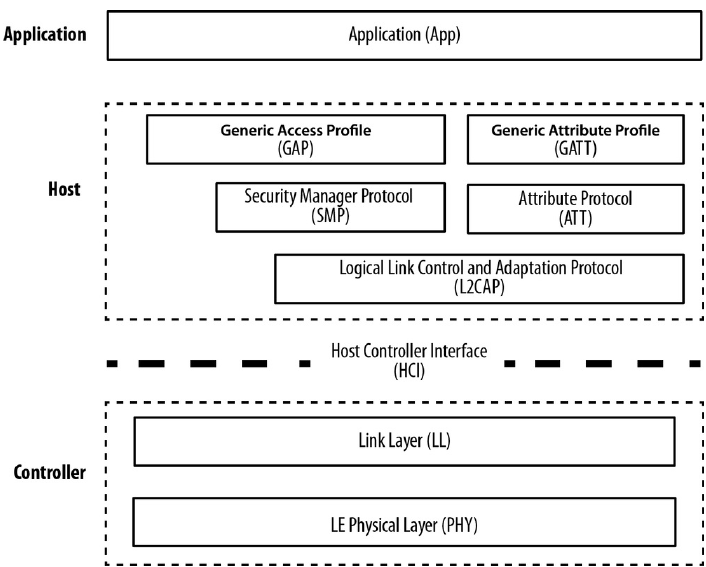
\includegraphics[width=0.9\linewidth]{\figdir/BLE_Protokolstack}
	\caption{\ac{ble} Protokollstack \cite[Seite 16]{Townsend14:GSB}}
	\label{FIG:protokollstack}
\end{figure}

\noindent In Abbildung \ref{FIG:protokollstack} ist der Protokollstack von \ac{ble} zu sehen. Dabei sind die drei Ebenen Controller, Host und Application zu erkennen. Auf der untersten Ebene liegt der Controller, in welchem das Physical Layer und das Linked Layer enthalten sind. Zwischen Host und Controller liegt das sogenannte \ac{hci}, welches die Schnittstelle zwischen den beiden Kommunikationspartnern darstellt. Im Host wiederum befinden sich sämtliche Protokolle und Profile, die notwendig sind, um Kommunikation zu ermöglichen. An der Spitze des Protokollstacks befindet sich die Applikation in der die Logik und Nutzerschnittstelle des aktuellen Anwendungsfalls liegt \cite[15]{Townsend14:GSB}. Wie diese einzelnen Komponenten funktionieren und untereinander kommunizieren, ist in den nachfolgenden Abschnitten erläutert.\\  


\subsection{Kommunikation}
\label{ss:funktionsweise:kommunkation}

Nachdem in Kapitel \ref{ss:funktionsweise:protokollstack} der allgemeine Aufbau von \ac{ble} erläutert wurde, wird im nachfolgenden Kapitel auf das Kernelement, die tatsächliche Kommunikation zwischen zwei oder mehreren Geräten von \ac{ble} eingegangen. Dabei werden drei Elemente im besonderen betrachtet: die Bekanntmachung, die Verbindung und der Datenaustausch.\\

\subsubsection{Advertisement}
\label{sss:funktionsweise:advertisement}

Das Advertsement, oder zu deutsch die Bekanntmachung, ist die Funktion, mittels welcher sich Geräte, die bereit sind, sich zu koppeln bei suchenden Geräten bekannt machen. Allerdings kann die Bekanntmachung auch für einen Broadcast von Daten ohne explizites Zielgerät verwendet werden.\\

\noindent Für das Advertisement sind drei der 40 Kanäle, in die der Frequenzbereich auf dem \ac{ism} Band unterteilt ist, reserviert. Ein Gerät kann diese Kanäle nutzen und ein Paket senden, welches verbindungsspezifische Daten bereitstellt. Generell gibt es folgende vier unterschiedliche Pakete, welche somit gesendet werden können:
\begin{itemize}
	\item{ADV\_IND}
	\item{ADV\_DIRECT\_IND}
	\item{ADV\_SCAN\_IND}
	\item{ADV\_NONCONN\_IND}
\end{itemize} 
Das "`ADV\_IND"' Paket sendet eine Bekanntmachung an alle Geräte, die zuhören und gibt bekannt, dass das Gerät bereit ist, sich mit jeglichem Gerät zu verbinden. Im Gegensatz dazu sendet das "`ADV\_DIRECT\_IND"' Paket eine direkte Nachricht an ein bestimmtes Gerät, dass es bereit ist, sich mit genau diesem zu koppeln. Um das zu gewährleisten, enthält die Payload des Paketes die beiden \ac{ble} Adressen der betroffenen Geräte. Diese beiden Pakete lassen auch zu, dass sich die Geräte miteinander verbinden. Die restlichen zwei Pakete lassen dies wiederum nicht zu. So ermöglicht das "`ADV\_SCAN\_IND"' Paket, lediglich einen Broadcast an alle hörenden Geräte zu senden, dass dieses Gerät in Reichweite ist. Es ist also sichtbar für die anderen Geräte. Um jedoch eine Verbindung einzugehen, müssen weitere Schritte unternommen werden. Das letzte Paket teilt allen Geräten in Reichweite mit, dass dieses Gerät nicht für eine Kopplung zu Verfügung steht. Alle Pakete bis auf das "`ADV\_DIRECT\_IND"' Paket können zusätzlich Daten enthalten, die über das Advertisement hinausgehen. Das ermöglicht auch den Einsatz von \ac{ble} Beacons, welche, ohne eine Verbindung einzugehen, Daten an alle Geräte in Reichweite senden können \cite{ADV:WWW}.\\

\subsubsection{Verbindung}
\label{sss:funktionsweise:verbindung}

Nachdem in Kapitel \ref{sss:funktionsweise:linked} erklärt wurde, wie Pakete aufgebaut sind und übertragen werden, gilt es noch zu erläutern, wie eine Verbindung in \ac{ble} abläuft, um diese Pakete tatsächlich transferieren zu können. Nachdem ein Central ein Gerät über das Advertisement gefunden hat, kann es eine Verbindungsanfrage initiieren. In diesem Paket sind drei wichtige Verbindungsparameter angegeben:
\begin{itemize}
	\item{Verbindungsintervall}
	\item{Slave Latenz}
	\item{Überwachungszeitüberschreitung}
\end{itemize}
Das Verbindungsintervall legt die Zeit fest, die zwischen zwei Verbindungsevents verstreicht. Eine Verbindung in \ac{ble} besteht ausschließlich aus derartigen Ereignissen und bleibt solange bestehen, wie diese regelmäßig stattfinden. Bei diesem Intervall gilt es abzuwägen, was wichtiger ist. Je geringer dieses Intervall ist, desto schneller ist die Verbindung. Jedoch verbraucht dieses Verhalten auch mehr Energie. Das Central muss also im Vorhinein festlegen, was für die kommende Verbindung wichtiger ist \cite{CON:WWW}. Die Slave Latenz legt die Nummer der Verbindungsevents an, die der Slave erlaubt ist, zu überspringen, bevor die Verbindung als beendet gilt. Ein weiterer Weg, wie eine Verbindung vorzeitig abgebrochen werden kann, wird durch die Überwachungszeitüberschreitung festgelegt. Bei dieser wird definiert, wie viel Zeit zwischen zwei erfolgreichen Übertragungen verstreichen darf. Sollte es also zu dem Fall kommen, dass über einen längeren Zeitraum erfolglos Pakete versendet werden, wird die Verbindung beendet \cite[Seite 23]{Townsend14:GSB}.\\

\begin{figure}[h]
	\centering
	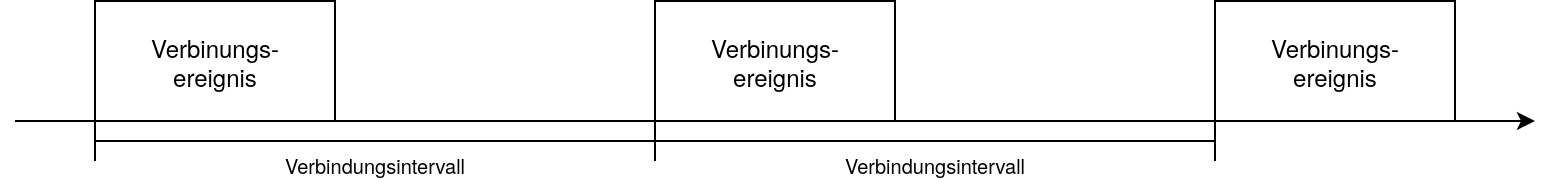
\includegraphics[width=\linewidth]{\figdir/ConEv}
	\caption{Ablauf einer \ac{ble} Verbindung \cite{CON:WWW}}
	\label{FIG:conenv}
\end{figure}

\noindent Wenn das Peripheral die Verbindung annimmt, wird diese, wie in Abbildung \ref{FIG:conenv} dargestellt, aufgenommen. Jedes dieser Ereignisse folgt einem bestimmten Ablauf: zuerst überträgt der Master eine Anfrage an den Slave. Dieser empfängt die Anfrage und verarbeitet diese. Anschließend sendet er eine entsprechende Antwort, die der Master empfängt. Wichtig dabei ist, das der Master nicht nur die Verbindung initiiert, sondern auch sämtliche Anfragen. Nachdem das definierte Verbindungsintervall abgelaufen ist, wird das nächste Verbindungsevent gestartet \cite{CON:WWW}.\\       

\section{Schnittstellenbeschreibung}
\label{s:interface} 

\subsection{SAP}
\label{ss:interface:sap}

\subsection{BLE}
\label{ss:interface:ble}

\subsection{Anbindungsmöglichkeiten}
\label{ss:interface:connect}

\subsubsection{Bewertung der Möglichkeiten}
\label{sss:interface:connect:eval}

\subsubsection{Administration}
\label{sss:interface:connect:admin}

\section{Vergleich mit anderen gängigen IoT Kommunikationsprotokollen}
\label{s:vergleich} 

\subsection{Vorteile}
\label{ss:vergleich:adv}

\subsection{Nachteile}
\label{ss:vergleich:disadv}

\section{Fazit}
\label{s:fazit}

  
%%% Local Variables: 
%%% mode: latex
%%% TeX-master: "thesis.tex"
%%% End: 
